% !TeX root = ../main.tex

\section{Problem Definition}
    \frame{\sectionpage}

    \begin{frame}{Seat Planning with Social Distancing}
      \begin{itemize}
      \item Group type $\mathcal{M} = \{1, \ldots, M\}$.
      \item Row $\mathcal{N} = \{1, \ldots, N\}$.
      \item The social distancing: $\delta$ seat(s).
      \item $n_i = i + \delta$: the new size of group type $i$ for each $i \in \mathcal{M}$.
      \item The number of seats in row $j$: $L_j^{0}, j \in \mathcal{N}$.
      \item $L_j = L_j^{0} + \delta$: the length of row $j$ for each $j \in \mathcal{N}$.
      \end{itemize}
      
      \begin{figure}[ht]
        \centering
        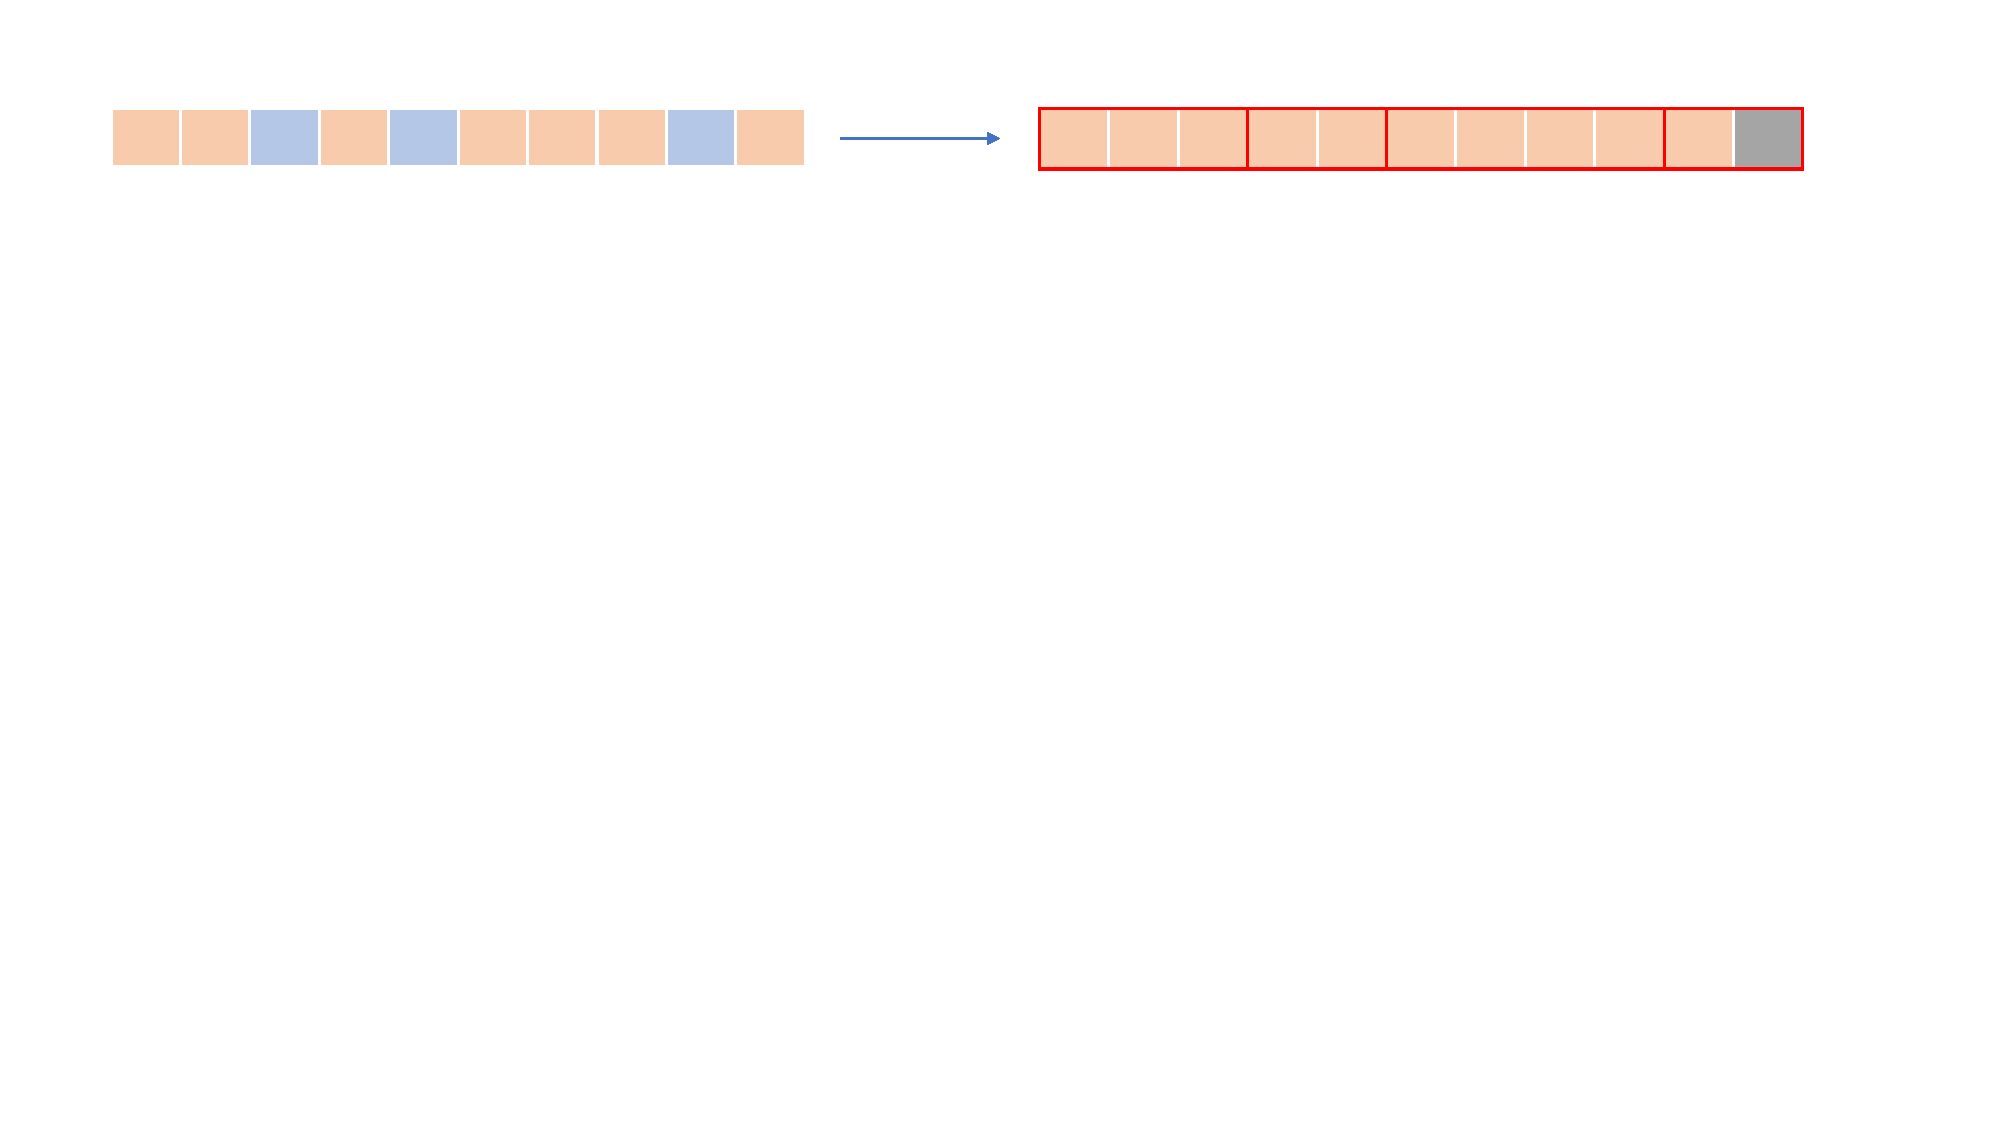
\includegraphics[width = 0.8\textwidth]{./images/dummy_seat.pdf}
        \caption{Problem Conversion with One Seat as Social Distancing}
    \end{figure}
    \end{frame}

  \begin{frame}{Basic Concepts}
    \begin{itemize}
      \item $\bm{h} = (h_1, \ldots, h_M)$, pattern, the seat planning for each group type in one row.
      Let $L = q(M + \delta) + r$.

      - The number of people accommodated: $|\bm{h}| = \sum_{i =1}^{M} i h_i = qM + \max\{r-\delta, 0\}$.
      
      - Loss for pattern $\bm{h}$: $L- \delta - |\bm{h}| = q \delta - \delta + \min\{r, \delta\}$.
      \item Largest patterns: $|\bm{h}| \geq |\bm{h}^{\prime}|$ for any $\bm{h}^{\prime}$. 
      \item Full patterns: $\sum_{i=1}^{M} n_i h_i = L$.
      \item[-] {\color{blue} Example}: 
      
      $\delta = 1$, $M =4$, $n_1 = 2, n_2 = 3, n_3 = 4, n_4 = 5$, $L = 21$.
      
      Largest patterns: $(0, 0, 0, 4), (0, 0, 4, 1), (0, 2, 0, 3)$.

      Largest may not be full: $(0, 0, 0, 4)$.

      Full may not be largest: $(1, 1, 4, 0)$.
    \end{itemize}
  \end{frame}

  \begin{frame}{Dynamic Seat Assignment Problem}
    \centering
    \small
    \begin{itemize}
    \item[-] There is one and only one group arrival at each period, $t = 1, \ldots, T+1$. 
    \item[-] The probability of an arrival of group type $i$: $p_i$.  
    \item[-] $\mathbf{L} = (l_1, l_2, \ldots, l_{N})$, where $l_j =0,\ldots, L_j, j\in \mathcal{N}$: Remaining capacity.
    \item[-] $u_{i,j}^{t}$: Decision. Assign group type $i$ to row $j$ at period $t$, $u_{i,j}^t =1$.
    \item[-] $U^{t}(\mathbf{L}) = \{u_{i,j}^{t} \in\{0,1\}, \forall i,j| \sum_{j=1}^{N} u_{i,j}^{t} \leq 1, \forall i, n_{i}u_{i,j}^{t}\mathbf{e}_j^{\top} \leq \mathbf{L}, \forall i,j \}$.
    \item[-] $\mathbf{e}_j^{\top}$: Unit row vector with $j$-th element being 1.
    \item[-] $V^{t}(\mathbf{L})$: Value function at period $t$, given remaining capacity, $\mathbf{L}$.
    \end{itemize}

    $$V^{t}(\mathbf{L}) = \max_{u_{i,j}^{t} \in U^{t}(\mathbf{L})}\left\{ \sum_{i=1}^{M} p_i ( \sum_{j=1}^{N} i u_{i,j}^{t} + V^{t+1}(\mathbf{L}- \sum_{j=1}^{N} n_i u_{i,j}^{t}\mathbf{e}_j)) + p_0 V^{t+1}(\mathbf{L})\right\}$$
    \small

    % \begin{itemize}
    %   \item[-] DP is computationally complex caused by the curse of dimensionality.
    %   \item[-] We give a seat planning by stochastic programming firstly, then apply stochastic planning policy to make the decision.
    % \end{itemize}
\end{frame}

\begin{frame}{Method Overview}
  \begin{itemize}
    \item Obtain seat planning composed of full or largest patterns.
    
    - Linear seat planning from stochastic programming
    
    - Integral seat planning from deterministic model

    - Construct largest or full patterns.

    \item Stochastic planning policy.

    - Group type control
% Tell us which group type should be broke which determines which rows can be placed. 

    - Assign The Group by Stochastic Values
% decide whether to accept 
% Both acceptance can decide 

  \end{itemize}
\end{frame}
